\section{Data}
\label{sec:sample}
The MaNGA (Mapping Nearby Galaxies at Apache Point Observatory; \citet{2015ApJ...798....7B}. [You have duplicated some text from the introduction.]

\subsection{Sample selection}
As described in the introduction post-starburst galaxies or PSB regions of galaxies can be identified from their spectra typically exhibiting the strong Balmer absorption lines of A-type stars. In addition, weak emmission lines of H$\alpha$ and [OII] emission lines indicate a quiescent state with little or no present star formation. 

The PSB sample employed in this work is that obtained from the sampling criteria adopted by Chen et al. (2019 in preparation, personal communication). This PSB sample is drawn from an analysis of 4633 galaxies made available as MPL-6 (SDSS MaNGA Product Launch 6). Following Chen et al. the following sample selection criteria for CPSBs and RPSBs must meet the following criteria:

\begin{itemize}
    \item Strong H$\delta$ absorption line features
    \item A strong 4000 \AA\ break 
    \item Weak or absent H$\alpha$ and [OII] emission lines
\end{itemize}

The PSB candidate selection process involves extracting  data from the MaNGA DAP output DAPTYPE MAPS-SPX-GAU-MILESHC: where SPX denotes individual spaxel binning; GAU a Gaussian fit algorithm to stellar spectra; and MILESHC is a reference to the MILES library \citep{2011A&A...532A..95F} of stellar spectrum templates, all as described in the MaNGA DR15 DAP documentation \citet{2019arXiv190100856W}. 
2-D maps provide the following data: 

\begin{itemize}
    \item Projected stellar rotation velocity
    \item Stellar velocity dispersion
    \item Ionised gas rotational velocity
    \item Ionised gas velocity dispersion
\end{itemize}

While the associated 3-D datacubes MAPS-VOR10-GAU-
MILESHC provide spatial spectral series yielding the following spectral properties across the galaxy field-of-view:

\begin{itemize}
    \item Dn4000 spectral index as a measure of the strength of the 4000 \AA\ break
    \item H$\delta_A$ absorption spectral index
    \item Nebular emission line equivalent widths
\end{itemize}

The H$\delta_A$ absorption spectral index is the equivalent width of H$\delta$ 4102\AA\ line as described by \citet{1994ApJS...94..687W}.

In addition to the above considerations, for a region of a galaxy to be considered as a PSB region at least 6 contiguous spaxels in the DAP analysis are required.

These selection criteria yields from the MaNGA MPL-6 dataset a total of 31 CPSBs and 37 RPSBS as listed in Tables \ref{tab:my-CPSBs} and \ref{tab:my-RPSBs} respectively. 

\begin{table}
\caption{Central-type PSBs identified in MaNGA MPL-6}
\label{tab:my-CPSBs}
\begin{tabular}{lccccc}
\hline
PlateIFU & RA & dec & z & log & S\'ersic\\
& & & & $M_*$ & n \\
\hline
7443-12701 & 230.50746 & 43.53234 & 0.020 & 9.693 & 4.43 \\
7964-1902 & 317.42261 & 0.62777 & 0.024 & 9.423 & 6.00 \\
8080-3702 & 49.22887 & -0.04201 & 0.023 & 9.877 & 5.91 \\
8081-3702 & 49.94685 & 0.62382 & 0.025 & 9.145 & 3.42 \\
8082-3704 & 50.88860 & -0.43854 & 0.024 & 9.761 & 2.51 \\
8143-3703 & 120.63984 & 42.39270 & 0.041 & 9.796 & 3.78 \\
8144-1902 & 114.45795 & 28.65289 & 0.016 & 8.799 & 1.48 \\
8313-6101 & 240.65805 & 41.29343 & 0.035 & 10.308 & 6.00 \\
8315-3703 & 236.16573 & 38.42536 & 0.076 & 11.025 & 5.54 \\
8331-6104 & 206.29627 & 42.31951 & 0.028 & 9.792 & 2.22 \\
8555-3701 & 246.76069 & 43.47610 & 0.046 & 10.601 & 3.82 \\
8623-9102 & 311.76380 & 0.43678 & 0.013 & 9.332 & 2.00 \\
8655-1902 & 358.46882 & -0.09873 & 0.022 & 9.241 & 1.82 \\
8713-3701 & 117.06113 & 39.04573 & 0.014 & 8.820 & 0.84 \\
8725-1902 & 127.48937 & 44.94016 & 0.043 & 10.513 & 4.05 \\
8933-3704 & 195.33050 & 27.86046 & 0.027 & 9.117 & 3.19 \\
8934-9101 & 196.26374 & 27.53704 & 0.022 & 9.086 & 6.00 \\
8935-12701 & 194.52342 & 29.01735 & 0.026 & 9.259 & 1.82 \\
8938-6102 & 120.06709 & 29.47144 & 0.045 & 9.823 & 3.34 \\
8941-3701 & 120.05960 & 26.69801 & 0.028 & 10.031 & 4.79 \\
8944-1902 & 148.42110 & 35.70188 & 0.040 & 9.590 & 5.93 \\
8950-3704 & 194.33162 & 27.61386 & 0.026 & 9.086 & 1.74 \\
8979-1902 & 242.58533 & 41.85490 & 0.040 & 10.634 & 6.00 \\
8996-3704 & 173.41287 & 52.67459 & 0.049 & 10.094 & 5.08 \\
8997-3703 & 170.72345 & 51.34178 & 0.034 & 9.600 & 1.25 \\
9047-3701 & 246.48074 & 25.41161 & 0.039 & 9.773 & 4.21 \\
9085-1902 & 260.61132 & 28.30970 & 0.069 & 10.662 & 6.00 \\
9493-12705 & 129.99929 & 23.41340 & 0.012 & 8.916 & 0.77 \\
9494-3701 & 126.75586 & 21.70675 & 0.015 & 9.949 & 1.96 \\
9494-3703 & 127.31796 & 23.80902 & 0.018 & 9.168 & 5.43 \\
9876-12701 & 194.63449 & 28.37796 & 0.020 & 8.851 & 5.05 \\
\hline
\end{tabular}
\end{table}

\begin{table}
\caption{Ring-type PSBs identified in MaNGA MPL-6}
\label{tab:my-RPSBs}
\begin{tabular}{lccccc}
\hline
PlateIFU & RA & dec & z & log & S\'ersic \\
& & & & $M_*$ & n \\
\hline
8080-3704 & 49.45745 & -0.55466 & 0.021 & 9.790 & 1.58 \\
8083-12703 & 49.92934 & 0.56548 & 0.024 & 9.960 & 3.80 \\
8085-6104 & 51.70891 & 0.19859 & 0.020 & 9.538 & 6.00 \\
8146-1901 & 117.05387 & 28.22509 & 0.027 & 9.907 & 1.71 \\
8250-6101 & 138.75315 & 42.02439 & 0.028 & 10.054 & 2.40 \\
8250-6104 & 140.41142 & 43.72615 & 0.040 & 10.383 & 1.47 \\
8255-3703 & 166.18780 & 45.15643 & 0.022 & 9.271 & 2.44 \\
8261-6103 & 181.54597 & 45.14921 & 0.067 & 10.583 & 4.76 \\
8262-3701 & 183.57898 & 43.53528 & 0.024 & 9.452 & 2.21 \\
8274-12701 & 164.58519 & 40.78823 & 0.026 & 9.314 & 0.85 \\
8322-1901 & 198.78425 & 30.40377 & 0.023 & 10.011 & 2.44 \\
8323-6103 & 196.10272 & 36.47995 & 0.023 & 9.858 & 1.35 \\
8439-6104 & 143.51035 & 50.02749 & 0.038 & 10.453 & 3.36 \\
8440-1901 & 136.11419 & 41.48621 & 0.024 & 9.067 & 2.20 \\
8440-6104 & 135.75897 & 40.43399 & 0.029 & 10.415 & 5.31 \\
8453-3704 & 154.48083 & 46.60329 & 0.030 & 9.782 & 1.78 \\
8458-6102 & 147.66431 & 44.33116 & 0.015 & 9.399 & 1.58 \\
8486-1901 & 238.44858 & 47.40496 & 0.019 & 9.226 & 1.39 \\
8547-9102 & 218.97634 & 53.39164 & 0.043 & 9.977 & 1.37 \\
8554-3701 & 183.00790 & 35.40440 & 0.024 & 9.657 & 2.67 \\
8604-3702 & 247.14945 & 39.71974 & 0.037 & 9.462 & 0.76 \\
8655-3701 & 356.75183 & -0.44739 & 0.071 & 10.729 & 3.34 \\
8932-12704 & 196.47287 & 28.11243 & 0.025 & 9.805 & 1.99 \\
8943-1901 & 154.97835 & 36.32574 & 0.026 & 9.854 & 3.10 \\
8950-12705 & 194.73314 & 27.83344 & 0.025 & 10.265 & 0.96 \\
8950-6101 & 194.76938 & 26.95819 & 0.027 & 9.137 & 2.66 \\
8982-6104 & 203.05706 & 26.94998 & 0.035 & 10.222 & 1.52 \\
8987-9102 & 137.98351 & 27.89927 & 0.047 & 10.080 & 1.45 \\
8997-3704 & 171.77902 & 51.13164 & 0.015 & 9.027 & 2.25 \\
9181-12705 & 120.55787 & 37.15008 & 0.084 & 10.664 & 1.68 \\
9184-3703 & 119.36531 & 33.25794 & 0.017 & 8.949 & 1.56 \\
9194-3702 & 47.02945 & 0.45621 & 0.074 & 10.623 & 4.82 \\
9487-9102 & 123.82033 & 46.07525 & 0.041 & 10.503 & 5.88 \\
9505-6102 & 139.17787 & 28.05423 & 0.028 & 9.708 & 1.15 \\
9868-3702 & 218.94756 & 47.00747 & 0.027 & 9.457 & 1.70 \\
9872-3701 & 233.23196 & 42.43826 & 0.020 & 9.745 & 2.28 \\
9891-6102 & 228.41485 & 28.24446 & 0.046 & 9.766 & 1.42 \\
\hline
\end{tabular}
\end{table}

\subsection{PSB spectra}
The spectrum of a PSB galaxy exhibiting central PSB features is shown in Figure \ref{fig:CPSB-8623-9102-spec}.
\begin{figure*}
    \centering
    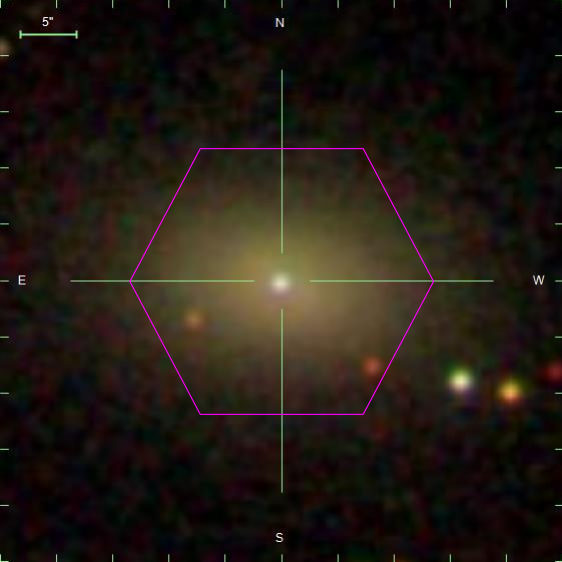
\includegraphics[width=0.22\textwidth]{images/Cutouts/CPSB-8623-9102-IM.png}
    \hfill
    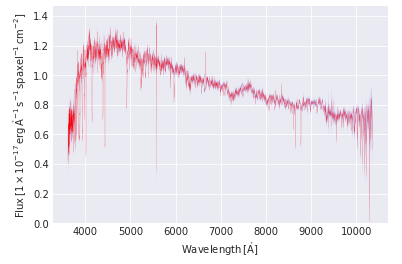
\includegraphics[width=0.38\textwidth]{images/Spectra/CPSB-8623-9102.png}
    \hfill
    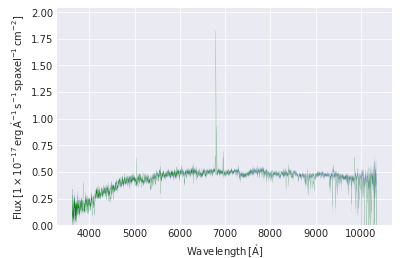
\includegraphics[width=0.38\textwidth]{images/Spectra/CPSB-CTRL-8990-3703-spec.png}
    \caption{Left: SDSS 3-colour image of central-type PSB 8623-9102. 
    Centre: The observed frame spectrum of the central spaxel of CPSB  8623-9102. Note the strong 4000 \AA\ break feature and strong hydrogen absorption lines in the wavelength region 3500 to 4500 \AA.
    Right: Observed frame spectrum of the control galaxy 8990-3703 with similar stellar mass to 8623-9102. This control galaxy shows relatively weak absorption lines and exhibits a strong H$\alpha$ emission line indicating the presence of cold gas and ongoing star formation.}
    \label{fig:CPSB-8623-9102-spec}
\end{figure*}


The spectrum of a ring-type RPSB galaxy exhibiting non-central PSB features is shown in Figure \ref{fig:RPSB-8323-6103-spec}.
\begin{figure*}
    \centering
    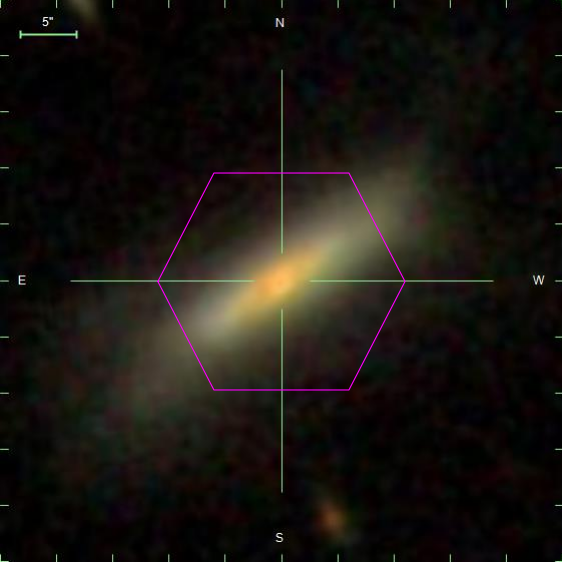
\includegraphics[width=0.24\textwidth]{images/Cutouts/RPSB-8323-6103-IM.png}
    \hfill
    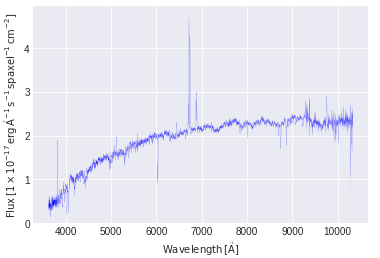
\includegraphics[width=0.35\textwidth]{images/Spectra/RPSB-8323-6103-27-27.png}
    \hfill
    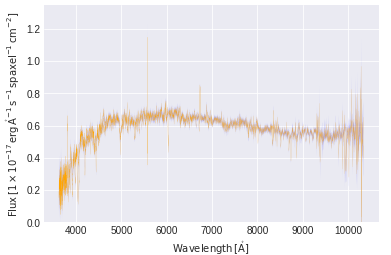
\includegraphics[width=0.35\textwidth]{images/Spectra/RPSB-8323-6103-34-32.png}
    \caption{Left: SDSS 3-colour image of the ring-type PSB 8323-6103. 
    Centre: The observed frame spectrum of the central region of ring-type PSB 8323-6103 at spaxel coordinates [27, 27] reveals strong H$\alpha$ emission consistent with an ample gas supply for continuing star formation.
    Right: The spectrum of ring-type PSB 8323-6103 at spaxel coordinates [34, 32], above and right of centre. The spectrum in this region exhibits the post-starburst features of weak emission lines, indicating a lack of gas, and strong Balmer absorption lines typical of the stellar atmospheres of A-type stars.}
    \label{fig:RPSB-8323-6103-spec}
\end{figure*}

An example of the MaNGA stellar velocity and gas velocity maps for a CPSB is illustrated in Figure \ref{fig:CPSB-8313-6101-VMAPS}.

\begin{figure}
    \centering
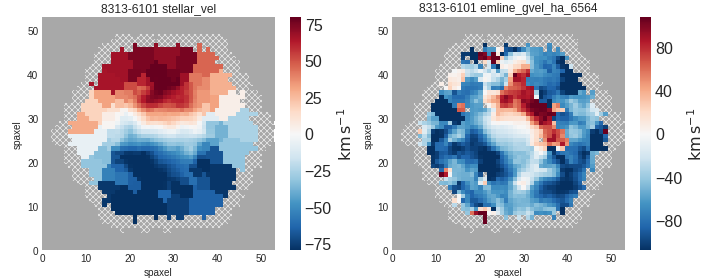
\includegraphics[width=\columnwidth]{images/VelocityMaps/CPSB-8313-6101-VMAPS.png}
    \caption{MaNGA velocity maps for CPSB 8313-6101: stellar velocity (left) and H$\alpha$ gas velocity (right).}
    \label{fig:CPSB-8313-6101-VMAPS}
\end{figure}

\subsection{Control galaxies}
Control galaxies as 'normal' galaxies not exhibiting PSB features. Also check this with Chen et al. (2019) for consistency.

\subsection{Quality screening}
Global kinematic velocity position angles (PA) for the sample were determined using the \texttt{fit\_kinemetry\_pa} routine as described in appendix C of \cite{2006MNRAS.366..787K}. The routine returns the angle of the line bisecting the greatest change in velocity between the receding and approaching sides. \cite{2019MNRAS.483..172D} performed a \texttt{kinemetry} analysis of over 8,000 galaxies from the internal MPL-8 release of the MaNGA survey. In order to obtain a clean sample of well defined global PAs they visually classified the stellar and H$\alpha$ gas velocity fields of all galaxies in their sample into 3 categories (Chris Duckworth, 2019, personal communication), and set flags in their dataset as follows:

\begin{itemize}
    \item [1] Dominant coherent rotation and well defined PA. 
    \item [2] Dominant coherent rotation but with complex motions or highly inclined velocity fields 
    \item [3] Do not use
\end{itemize}

During this analysis galaxies with kinematically decoupled cores (KDCs) and warped velocity fields were also identified.

TODO: This is where the nesting error ocurred. Find out why?

The resulting MPL-8 dataset  \cite{2019MNRAS.483..172D} dataset of galaxies with reliable global PAs (flagged as [1] or [2]) was matched with the PSB galaxies in the sample of Chen et al. (2019, in prep.) to obtain a subset of PSBs with good \texttt{kinemetry} analysis flags. Furthermore a subset of those PSBs with $\Delta$PAs > 30\textdegree\ was extracted. The results are shown in Tables \ref{tab:my-CPSBs} and \ref{tab:my-RPSBs}. 

[Include a few examples of the PDF output from kinemetry: Chris' plots.]

In classical Kinemtry analysis it is considered significant if the $\Delta$PA position angle is greater than 30 degrees. We show some examples of misaligned stellar and gas velocity fields here: 
[TODO: tidy up this section.]

\begin{figure}
    \centering
    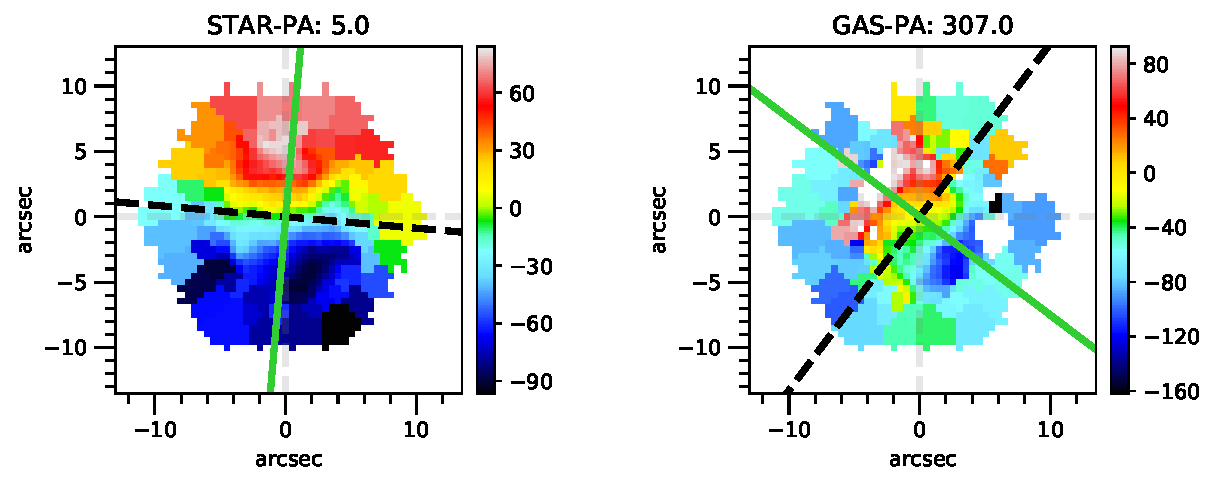
\includegraphics[width=\columnwidth]{images/PAplots/PAplotsCPSB/8313-6101-PA.pdf}
    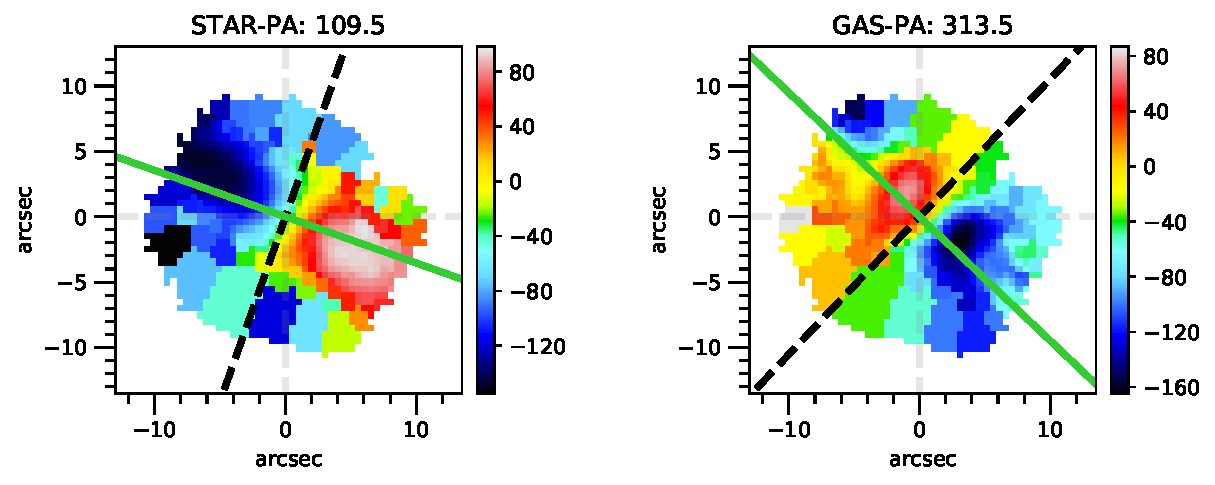
\includegraphics[width=\columnwidth]{images/PAplots/PAplotsRPSB/8323-6103-PA.pdf}
    \caption{Kinemetry-derived position angles (PA) for stellar velocity (left) and gas velocity (right) of two PSB galaxies exhibiting a significant $\Delta$PA. Top: CPSB 8313-6101, and bottom: RPSB 8323-6103. The velocity position angle is displayed as the green solid line while the black dashed line denotes the bisector of the velocity field between the receding (red) and blue (approaching) sides. The velocity colour scale is \kms. Credit for data analysis and plots: Chris Duckworth}
    \label{fig:CPSB-8313-6101-PA}
\end{figure}

\begin{table}
\caption{CPSBs with PA offset \textgreater 30 deg.}
\label{tab:offsetCPSBs}
\begin{tabular}{lccc}
\hline
PlateIFU  & Stellar PA & H$\alpha$ PA & $\Delta$PA \\
  & (deg.) & (deg.) & (deg.) \\
\hline
8313-6101 & 5 & 307 & 58 \\
8655-1902 & 335 & 127 & 152 \\
8725-1902 & 22 & 175 & 153 \\
8938-6102 & 214 & 47.5 & 166.5 \\
9494-3701 & 140.5 & 243 & 102.5 \\
\hline
\end{tabular}
\end{table}

\subsection{PA plots: misaligned RPSBs}

\begin{table}
\caption{RPSBs with PA offset \textgreater 30 deg.}
\label{tab:offsetRPSBs}
\begin{tabular}{lccc}
\hline
PlateIFU   & Stellar PA & H$\alpha$ PA & $\Delta$PA \\
  & (deg.) & (deg.) & (deg.) \\
\hline
8080-3704 & 24 & 154 & 130 \\
8262-3701 & 153.5 & 118.5 & 35 \\
8323-6103 & 109.5 & 313.5 & 156 \\
8439-6104 & 5.5 & 107 & 101.5 \\
8453-3704 & 44 & 91 & 47 \\
8486-1901 & 295.5 & 85 & 149.5 \\
8554-3701 & 250 & 68 & 178 \\
8932-12704 & 166.5 & 134.5 & 32 \\
9872-3701 & 208.5 & 81 & 127.5 \\
\hline
\end{tabular}
\end{table}

